\title{High Performance Genetic Algorithms for Steganalysis}
\author{
Joseph Charles Bingham \\
Department of Mathematics\\
Iowa State University of Science and Technology\\
Ames, Iowa 50010, United States of America \\
jbingham@iastate.edu
}
\date{\today}
\documentclass[12pt]{article}
\usepackage{graphicx}
\usepackage{amssymb}
\usepackage{listings}
\usepackage{xcolor}
\graphicspath{ }
\begin{document}
\maketitle

\begin{abstract}
\par This research outlines a novel implementation of a genetic algorithm that leverages high performance parallelizations to detect 
steganaraphically embedded images. The two main components that are new to this project are the application of parallelization for genetic algorithms and the application of genetic algorithm for steganalysis for LSB embedding. Typical steganalytic methods which use machine learning techniques require an unreasonable amount of pre-classified data and copious amounts of time for training the engine. The data needed for such operation usually must be lab generated, which can lead to the biases when compared to real world, and often is constrained to specific parameters, such as they must remain within either the spacial domain or the JPEG domain, must be the same pixel width, etc., making these engines limited to what image space they detect over. The need for all data to be used in training the engine, as well as the linear nature of the engines used precludes them from being parallelized in any meaningful fashion. 
\par This new algorithm does not succumb to these shortfalls. By using solution sets of pixels as the data which the genetic engine trains over, and fixing the image(s) under suspicion, the engine can be parallelized, vastly increasing the efficiency. Since the algorithm searches for sets solutions and then uses a fitness function to determine whether the findings were significant using a known statistical test, it does not require training data at all, mean that there are no biases introduced by lab generated data. The algorithms flexibility does not limit it to just one format of images, meaning that the same program can be used without the need to generate a new set of data or train a new engine. 
\end{abstract}

\section{Background Information}
\paragraph{Steganography and Steganalysis}
\par Steganography is the practice of embedding information into photographs or audio media in such a way that it is not detectable to the average person. The form of steganography that the scope of this project is most interested in is LSB (Least Significant Bit) embedding of images using random paths [1].
\par This, as the name suggests, is where the path of the embedding stream is random in nature. When a pixel from the image is selected to be altered, the least significant bit is overridden to be the same as the next bit in the embedding stream. Since it is just the least significant bit, very little visual alterations occur. This makes detection difficult, if not impossible without the aid of software. (Example below) \\
\begin{center}
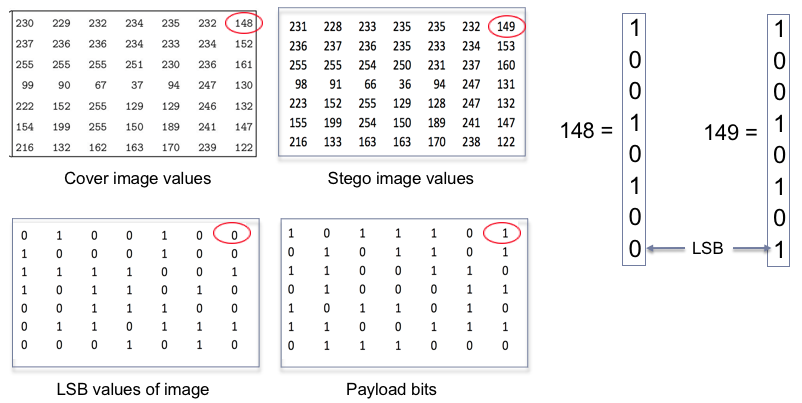
\includegraphics[scale=.5]{LBS.png}
\end{center} 
\par A random embedding path in steganography implies that the pixels whose bits are overwritten in the above fashion are chosen at random.
\par Steganalysis is the discovery of the existence of hidden information; therefore, like cryptography and cryptanalysis, the goal of steganalysis is to discover hidden information and to break the security of its carriers [2].
\paragraph{Genetic Algorithms}
\par Genetic Algorithms are algorithms that follow a specific machine learning paradigm [3]. They are classified by their similarity to natural selection as found in evolution in the wild. They consist of three main parts: a cost function, a tester bot, and a builder bot.
\par The cost function determines the viability of each solution. Typically this function determines how well the solution completes the task that is trying to be accomplished, and is usually from ${\rm I\!R}^n \mapsto [0, 1]$. 
\par The tester bot tests each solution based on the cost function. Its job is to determine what the value of the test function and to rank each solution.
\par The builder bot takes each the best solutions, as ranked by the tester bot, generates more solutions based on their attributes. It generates the new solutions by randomly modifying the best solutions to descend along the gradient of the solution space to an optimal (minimal cost) solution.

\section{Implementation :: Theory}
\paragraph{Assumptions}
\par The assumptions that are made for this research are :
\\ 1. The bit stream that is generated by the message has an equal amount of 0's as it does 1's. This is reasonable as the message is likely encrypted using some hash function, which would likely convert the message to a binary string with a uniform distribution of 0's and 1's.
\\ 2. The path of embedding is uniform random, meaning that each pixel is equally likely to have received a bit from the bit stream. This implies that each groups of pixels of equal size likely contains an equal number of overwritten bits. This is a reasonable to assume as there already exist many techniques for finding embedding paths which are not random. 
\\ 3. The message overwrites 50\% of the image. For theoretical purposes, this makes the computation easier, but for the practical aspects, this embedding rate is enough to detect with most methods, and would provide a good benchmark for the algorithm.
 
\paragraph{Genetic Algorithm for Steganalysis}
\par One of the novel components to this research is the use of genetic algorithm for steganalysis. The thought behind this is to generate a classifier for steganographically embedded images versus normal cover images.
\par This is done by creating a evolutionary solution for a path finding algorithm. The path finding algorithm optimizes the possible paths of embedding to determine the probability of payload being embedded. If the genetic algorithm's internal weight function is triggered, then the probability along the path found was deemed high enough to consider the image having a payload embedded.
\par The weight function is the $\chi ^ 2$-attack from steganalysis [4]. The basis of this attack is that grey scale values that differ by only the last bit (the bit that is overwritten) would show up equally in the embedding path. This is because an LSB within the embedding path has an equal likelihood of being 0 or 1.
For example: \\
An image, I, whose pixels are represented by 3 randomly generated bits in the following matrix : 
\begin{center}
$  \left[ \begin{array}{cccc} 
 101 & 011 & 111 & 100\\
  001 & 001 & 100 & 001\\
 101 & 110 & 010 & 101 \\
 101 & 110 & 010 & 101 \\  \end{array} \right] $ 
\end{center}
with a lexicographical embedding of the message stream 
\begin{center}
$ \left[ \begin{array}{c} 1,  0 , 1,  0,  1,  0,  1,  0,  1,  0,  1,  0,  1,  0,  1,  0 \end{array} \right] $
\end{center}
becomes I'

\begin{center}
 $ \left[ \begin{array}{cccc}
 101 & 010 & 111 & 100\\
  001 & 000 & 101 & 000\\
 101 & 110 & 011 & 100 \\
 101 & 110 & 011 & 100 \\  \end{array} \right] $ 
\end{center} 
\newpage This gives the histograms, \\ \\  
\begin{center}
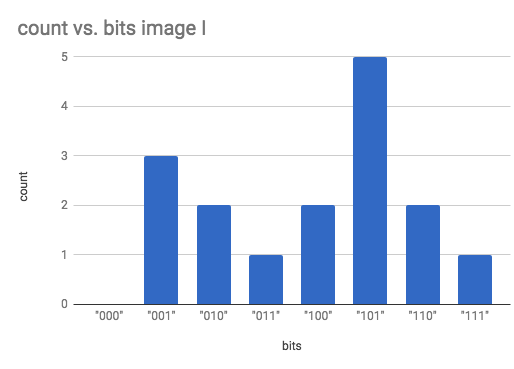
\includegraphics[scale=.45]{histogramI.png} 
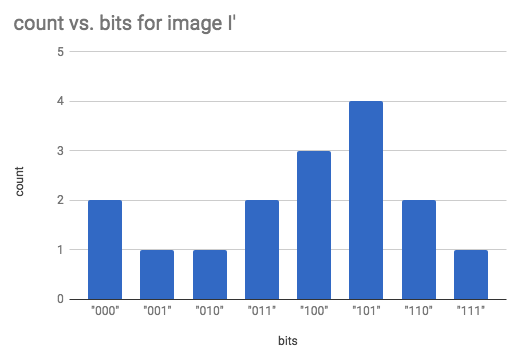
\includegraphics[scale=.45]{histogramIprime.png} 
\end{center}
\par As one can see, the values before the embedding, I, are far less pairwise normalized than those in I'. By feeding these pairwise differences into the cumulative distribution function for the $\chi^2$ distribution, with the degree of freedom equal to the number of bins in the sample set, we get a value that is between 0 and 1, and is directly correlated to how likely it is that the pixels are stegonagraphically embedded. This provides us with a function 
$ F : {\mathbb{Z}_{2^k}^{n^2}} \mapsto [0, 1] $, where k is the number of bits to represent the grey scale value and $ n \times n $ is the square pixel array size of the image in pixels. For the above example, k = 3 and n = 4. This provides a natural candidate for use as a fitness function.
\par The tester bot goes through each solution of pixels and evaluates them based on this fitness function, and ranks them on this value. A key difference between this genetic algorithm and other genetic algorithms is that the typical actor of the data over which the genetic algorithm would be the images that are under suspicion. However, in this algorithm, the data is the solution set and the image is fixed. This allows for a much more compact implementation with regards to memory as each solution would only need to keep track of the pixels it is referencing, and not all of the images. 
\par For testing the functions, the bot not only tests the overall fitness of the total solution, but it also chunks the solution into four, with the first fourth being the pixels of the solution which lie within the first quarter of the image lexicographically, the second fourth being from the second fourth of the image and so on. The bot then evaluates the fitness of each chunk. (Sample below). 
\\ \\
 $ \left[ \begin{array}{cccc}
 101 & 010 & 111 & 100\\
  001 & 000 & 101 & 000\\
 101 & 110 & 011 & 100 \\
 101 & 110 & 011 & 100 \\  
 \end{array} \right]  \mapsto 
 \left[ \begin{array}{cccc}
 101 & 010 & 111 & 100\\
 \hline
  001 & 000 & 101 & 000\\
 \hline
 101 & 110 & 011 & 100 \\
 \hline
 101 & 110 & 011 & 100 \\  
 \end{array} \right] \mapsto
 \left[ \begin{array}{c}
 $ fitness val 0 $ \\
 \hline
 $ fitness val 1 $ \\
 \hline
$ fitness val 2 $ \\
 \hline
$ fitness val 3 $ 
 \end{array} \right] \\
 $

\par The philosophy of the builder bot for this implementation is to combine two solutions based on their fitness scores in such a way that gives priority to pixels that appear in both, then pixels from the solution with the higher fitness, then random pixels from the same section of the image (to add nondeterminism into the solutions). This is done by taking the intersection of the two sets, add these to the new solution. Then adding the amount determined by the ratio of the two fitness values from remainder of the pixels from each solution. Then randomly changing up to one pixel. This will have the solutions converge to the highest fitness value, which is used to determine whether the image has been embedded. 

\paragraph{Parallel Implementation of Genetic Algorithms}
\par The other novel component is the parallelization of the genetic
algorithms to speed up the training time of the evolutionary model. The reason this project requires a parallel training model, as opposed to a serial implementation is, because the quantity of data (the solution sets) that needs to be ingested by the engine is immense, O($n^8$), where n is the side length of the image in pixels.
\par The parallelization is achieved by using a "island" inspired model. This is where each node of the cluster getting its own evolutionary model, but with the same cost function. Then after some number of iterations, the nodes give each other their top solutions to reproduce with the other solutions. This speeds up, and aids with, the convex optimization.
\par The parallelization comes in two flavors. The first is multiprocessing, which is the running of two or more programs or sequences of instructions simultaneously by a computer with more than one central processor. This creates the "islands", where each node is running the genetic algorithm independently, going though their own evolution in isolation, and then syncing up to swap their best solutions. This allows for multiple gradient descents which makes it more likely that the global minimum is found. This research uses MPI for this.
\par The other type of parallelization that will be used is multithreading. Multithreading is a technique by which a single set of code can be used by several processors at different stages of execution. This will be used within each process to optimize operations, such as creating the next generation of solutions. This research uses Open MP for this. 


\section{Implementation :: Code}
This section includes some highlights of the code implementation, along with the mathematical reasoning and proofs of their complexities.
\lstset { 
    language=C++,
    basicstyle=\footnotesize,
}
\begin{lstlisting}
/*
gamm:
param: double x, input to function
return: double, the gamma function applied
implemented using an approximation.
This was an approximation using a rational approximation found by SCHMELZER
and TREFETHEN
The memory complexity of this is O(1) and time complexity of O(1)
*/
double gamm(double x) 
{
    double ret = (1.000000000190015 + 
                 76.18009172947146  / (x + 1) +  
                 -86.50532032941677 / (x + 2) + 
                 24.01409824083091  / (x + 3) +  
                 -1.231739572450155 / (x + 4) + 
                 1.208650973866179e-3/ (x + 5) + 
                 -5.395239384953e-5 / (x + 6));
    
    return ret * sqrt(2.0*PI)/x * pow(x + 5.5, x+.5) * exp(-x-5.5);
}
\end{lstlisting}
By an easy inspection, the memory complexity of this is O(1) and time complexity of O(1), as there is no dynamically allocated memory, nor are there any loops [5].

\lstset { 
    language=C++,
    basicstyle=\footnotesize,
}
\begin{lstlisting}
  Solution *mixSolutions(Solution *other)
  {
   Solution *ret = new Solution;
   for(int i = 0; i < 4; i++)
   {
    if(this->fitVal[i] >= other->fitVal[i])
    {
     int k = 0;
     int T[SOL_SIZE * 2] = {0};
     for(int j = 0; j < SOL_SIZE; j++)
     {
      T[this->values[i][j]]++;
      T[other->values[i][j]]++;
     }
     for(int j = 0; j < SOL_SIZE*2; j++)
     {
      if(T[j] == 2)
      {
       ret->values[i][k] = T[j];
       k++;
      }
     }
     int upperLim = (SOL_SIZE - k)*(this->fitVal[i]/other->fitVal[i]);
     while(k < upperLim)
     {
      for(int l = 0; l < SOL_SIZE; l++)
      {
       if(!in(this->values[i][l], ret->values[i])
       {
        ret->values[i][k] = this->values[i][l];
        k++;
        break;
       }
      }
     }
     while(k < SOL_SIZE)
     {
      for(int l = 0; l < SOL_SIZE; l++)
      {
       if(!in(other->values[i][l], ret->values[i])
       {
        ret->values[i][k] = other->values[i][l];
        k++;
        break;
       }
      }
     }
    }
    else
    {
     int k = 0;
     int T[SOL_SIZE * 2] = {0};
     for(int j = 0; j < SOL_SIZE; j++)
     {
      T[this->values[i][j]]++;
      T[other->values[i][j]]++;
     }
     for(int j = 0; j < SOL_SIZE*2; j++)
     {
      if(T[j] == 2)
      {
       ret->values[i][k] = T[j];
       k++;
      }
     }
     int upperLim = (SOL_SIZE - k)*(this->fitVal[i]/other->fitVal[i]);
     while(k < upperLim)
     {
      for(int l = 0; l < SOL_SIZE; l++)
      {
       if(!in(this->values[i][l], ret->values[i])
       {
        ret->values[i][k] = this->values[i][l];
        k++;
        break;
       }
      }
     }
     while(k < SOL_SIZE)
     {
      for(int l = 0; l < SOL_SIZE; l++)
      {
       if(!in(other->values[i][l], ret->values[i])
       {
        ret->values[i][k] = other->values[i][l];
        k++;
        break;
       }
      }
     }
    }
    int a = rand();
    if((a %= 400) < 4 && !in(a, ret->values[i])
    {
     ret->values[i][a] = ret->values[i][rand() % (SOL_SIZE)];
    }
   }
   return ret;  
  }
\end{lstlisting}
\par Looking at the call to in() , which is implemented in a O(n) fashion (where n is the number of pixels), it is within a for loop within a while loop within a for loop, giving this step O($n^4$). Although this is much larger than the typical highest complexity of O($n^2$) for industry applications, this is much better than the O($2^n$) of the CNN used by most steganalytic applications.  
\section{Results}
\quad In comparison to brute force searching, which would have a work case of $ {  { n^2 } \choose  { { n^2 } \over 2 } } $ where n is the side length in pixels, which would be looping though every possible combination of pixels, this algorithm, assuming that only half of the solution pixels need to be found, would only need a fraction of that. 
\par This project results in the creation of a detection algorithm for steganalysis which can be applied to not just fixed patterns of embedding, but random paths of embedding. This has also provided a frame work for parallelizing more general genetic algorithms

\section{Next Steps}
\paragraph{Relieving the 50\% embedding requirement}
\par One thing that I wish to experiment with is adding a random chance that with each new generation a pixel could either randomly be added or removed from each of the four segments. This could theoretically account for more embedding rates than just 50\%. However, this makes the complexity much higher, and it may be more efficient to loop though each suspected embedding rate.
\paragraph{Implementing the algorithm for colored photos}
\par This should be an easy extension, but the multicolor pixel values add a new layer of complexity that may require a different approach to the parallelization and distribution of pixels for each solution. Another layer of complexity that this may add is the growth in the number of bins, which would require either a higher embedding rate or larger photos to be able to reliably utilize the $\chi ^2$ attack.
\paragraph{Experimenting with a different number of sections}
\par This would allow for the path to be more refined and could increase accuracy, however the smaller the section are, the less likely the $\chi ^2$ attack will be able to use the data constructively. This means that the images would have to contain more pixels, or there would need to be less values that could map to, to reduce the number of bins,

\section{Bibliography}
$[1]$ Yu, L., Zhao, Y., Ni, R. et al. EURASIP J. Adv. Signal Process. (2010) 2010: 876946. https://doi.org/10.1155/2010/876946 \\
$[2]$ Deborah Radcliff "Computer World" http://www.computerworld.com/securitytopics/security/story/0,10801,71726,00.html \\
$[3]$ Whitley, D. Stat Comput (1994) 4: 65. https://doi.org/10.1007/BF00175354 \\
$[4]$ Orion.math.iastate.edu. (2018). Pairs of Values and the Chi-squared Attack. https://orion.math.iastate.edu/dept/thesisarchive/MSCC/CStanleyMSSS05.pdf. \\
$[5]$ Schemelzer and Trefethen, SIAM J. NUMER. ANAL, Computing the Gamma Function Using Contour Integrals and Rational Approximations (2007) https://doi.org/10.1137/050646342
\end{document}

